\section{Theoretical background}

\subsection{Overview of Adaptive Testing in Psychophysics}

\subsection{Bayesian statistics}

In Bayesian statistics \textit{probability} is defined epistemologically: probability distributions are used to formalize what we \textit{know} of something. Another distinctive feature is that we begin from a formalization of \textit{prior} knowledge that is updated by making observations. 

As a simple example we know that in an unmodified deck of cards there's uniform probability for a random card to be any of the four suits. We can represent this with a uniform discrete distribution as in the left panel of Figure \ref{fig:suitsDiscUnif}

\begin{figure}[htb]
	\begin{center}
		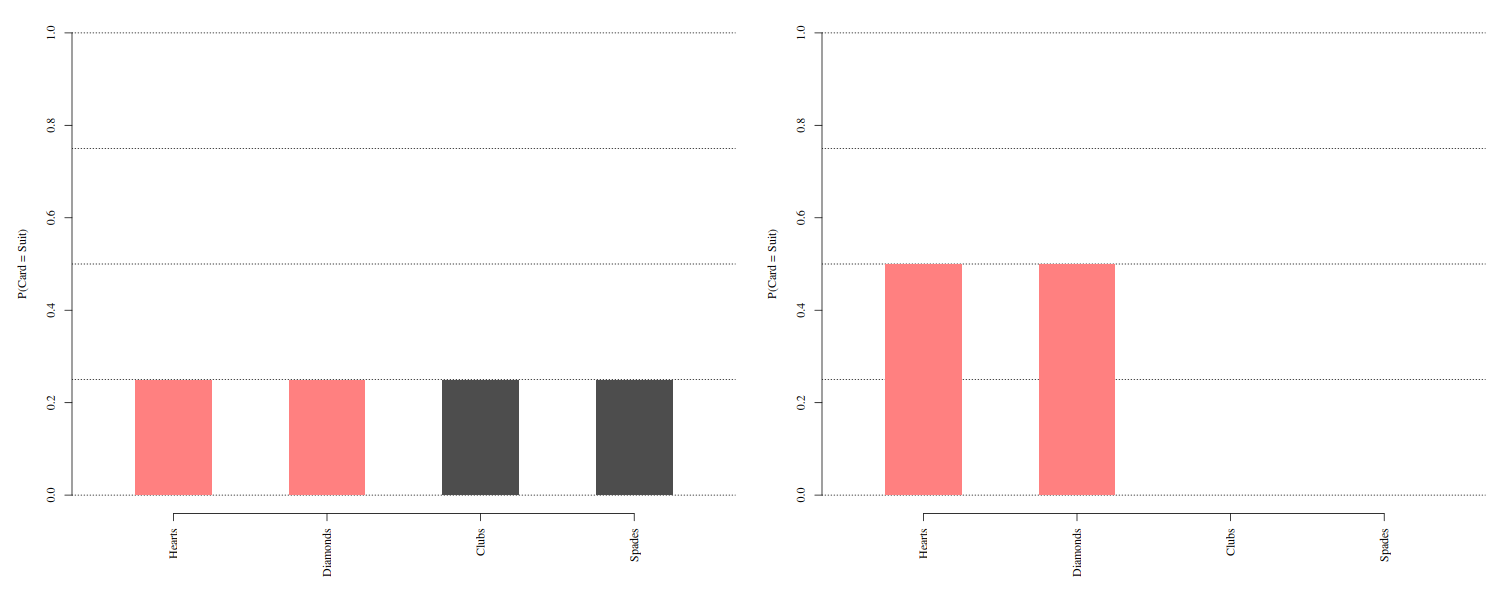
\includegraphics[width=5in]{Parts/TheoreticalBackground/Figs/discrBayes.png}
	\end{center}
	\caption{}
	\label{fig:suitsDiscUnif}
\end{figure}	

If our interrogator presents us with the knowledge that the card is red, we can update our knowledge. Now the probability of the card being clubs or spades is zero, and the probability of the card being hearts or diamonds is equal, see the right panel of Figure \ref{fig:suitsDiscUnif}. 



\begin{figure}[htb]
	\begin{center}
		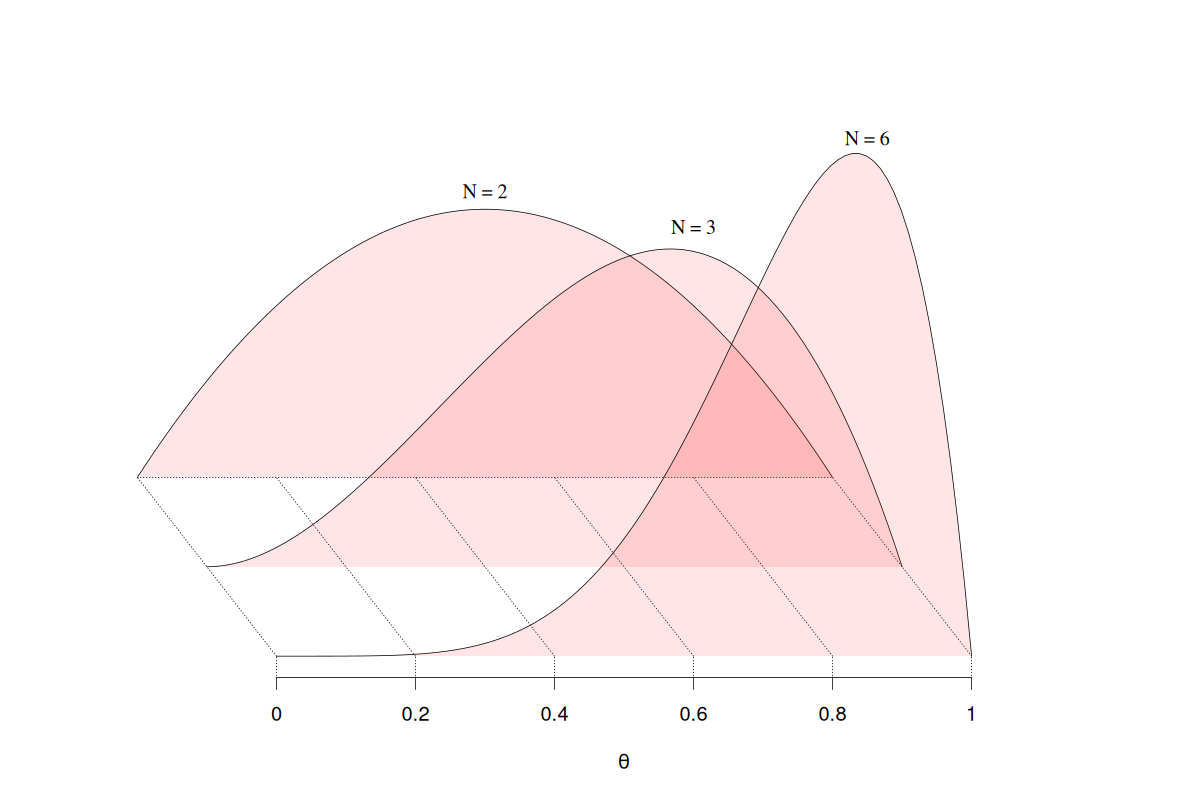
\includegraphics[width=4in]{Parts/TheoreticalBackground/Figs/sequentialBeta.png}
	\end{center}
	\caption{Demonstration of how uncertainty is reduced as more data is observed. Plausible values for the parameter $\theta$ become more and more concentrated.}
\end{figure}

\subsection{Markov Chain Monte Carlo}

\subsection{Likelihood Free Bayesian Estimation}

\subsection{Introduction to Bayesian Adaptive Testing}

\subsection{Likelihood Free Adaptive Testing}

\subsection{Entropy}

Entropy of a continuous distribution is

\begin{equation}
h[f(x)] = \int f(x)\log f(x)
\end{equation}

ERROR REFERENCE

In the continuous case we have to integrate over the 

\begin{equation}
ig(x) = h \left(\int p(y) \right)  - \int h \left( p(y) \right) 
\end{equation}

In discrete case the integrals become summations:

\begin{equation}
	ig(x) = h \left(\sum p(y) w(x)\right)  - \sum h \left(p(y)w(x)\right) 
\end{equation}

and, of course, given an IID sample, we can divide the sums with N to get the expectations:


\section{Black box algorithm}

In principle, the proposed framework could be implemented as a black box algorithm that could be used to optimize the data acquisition for any model (as defined in this thesis).